%!TEX root = ../Final_Assignment_SP_ML4IM_2023.tex
\chapter{Results}
\label{ch:results}

% ausführlich
% NOT FINAL - unsure about section structure and names
% alle

The results of the project are presented in this chapter. For that, the results of the different approaches to preprocess the data before they were used for training are presented and compared. This chapter will take a look at the results one by one.

% RGB
First af all the results of the default RGB training are presented. The default RGB training was done using the raw RGB data without any preprocessing. The results of this training are shown in Table~\ref{fig:results_rgb}.

\begin{figure}[htbp] 
    \centering
    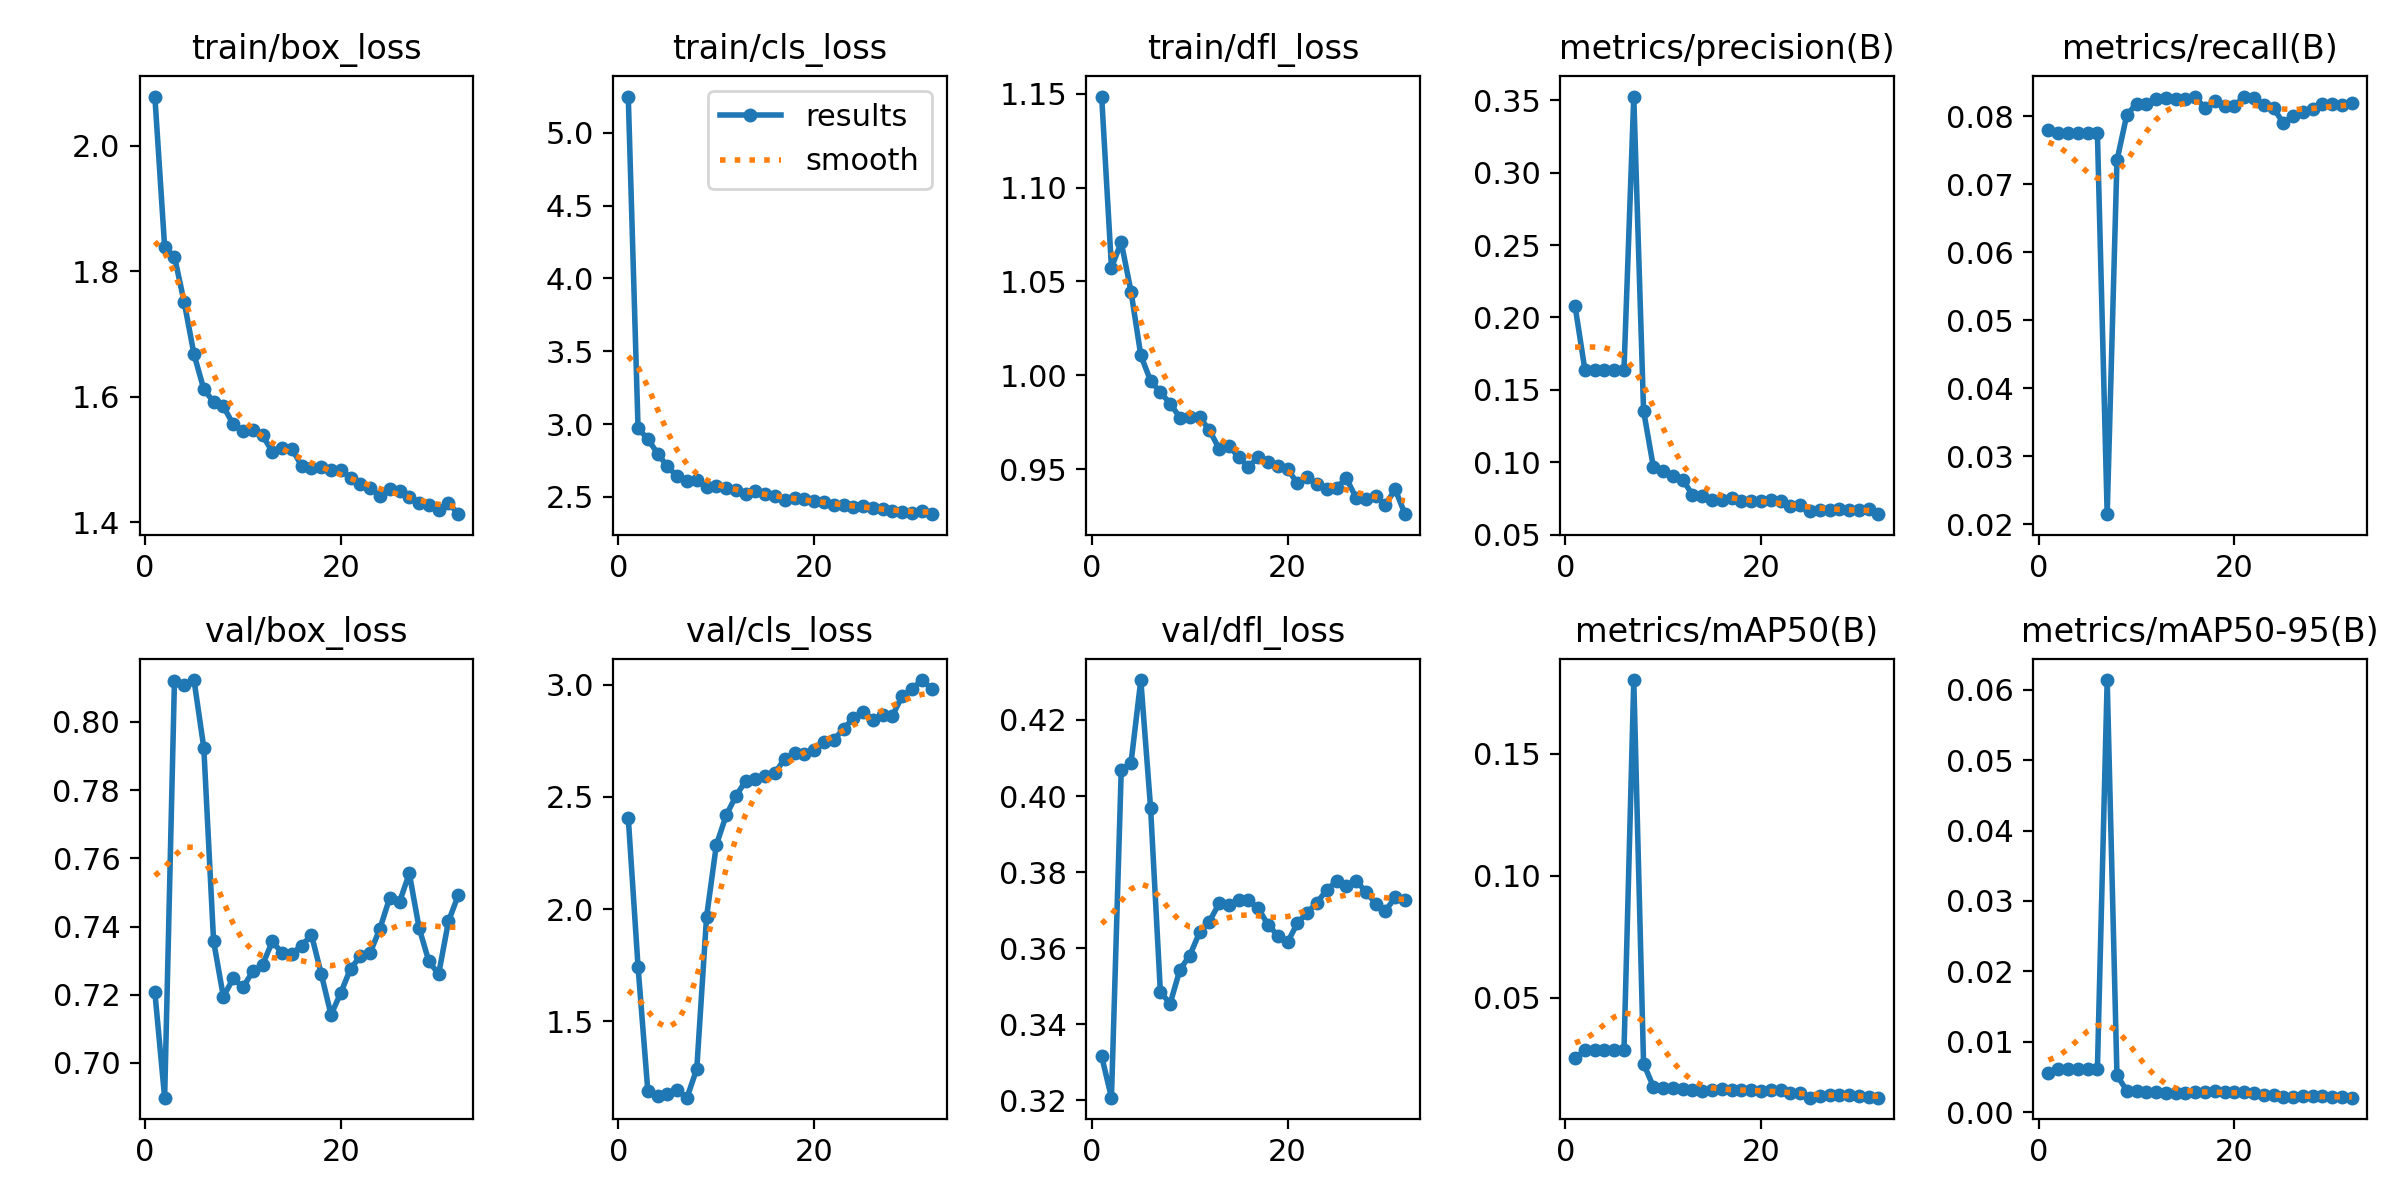
\includegraphics[width=0.75\textwidth]{images/results/rgb_results.png}
    \caption{Results of the model training with RGB data}
    \label{fig:results_rgb}
\end{figure}

% TODO results of rgb

% HSV
The next results are from the training with the HSV data. The HSV data was created by converting the RGB data to the HSV color space. The results of this training are shown in Table~\ref{fig:results_hsv}.

\begin{figure}[htbp] 
    \centering
    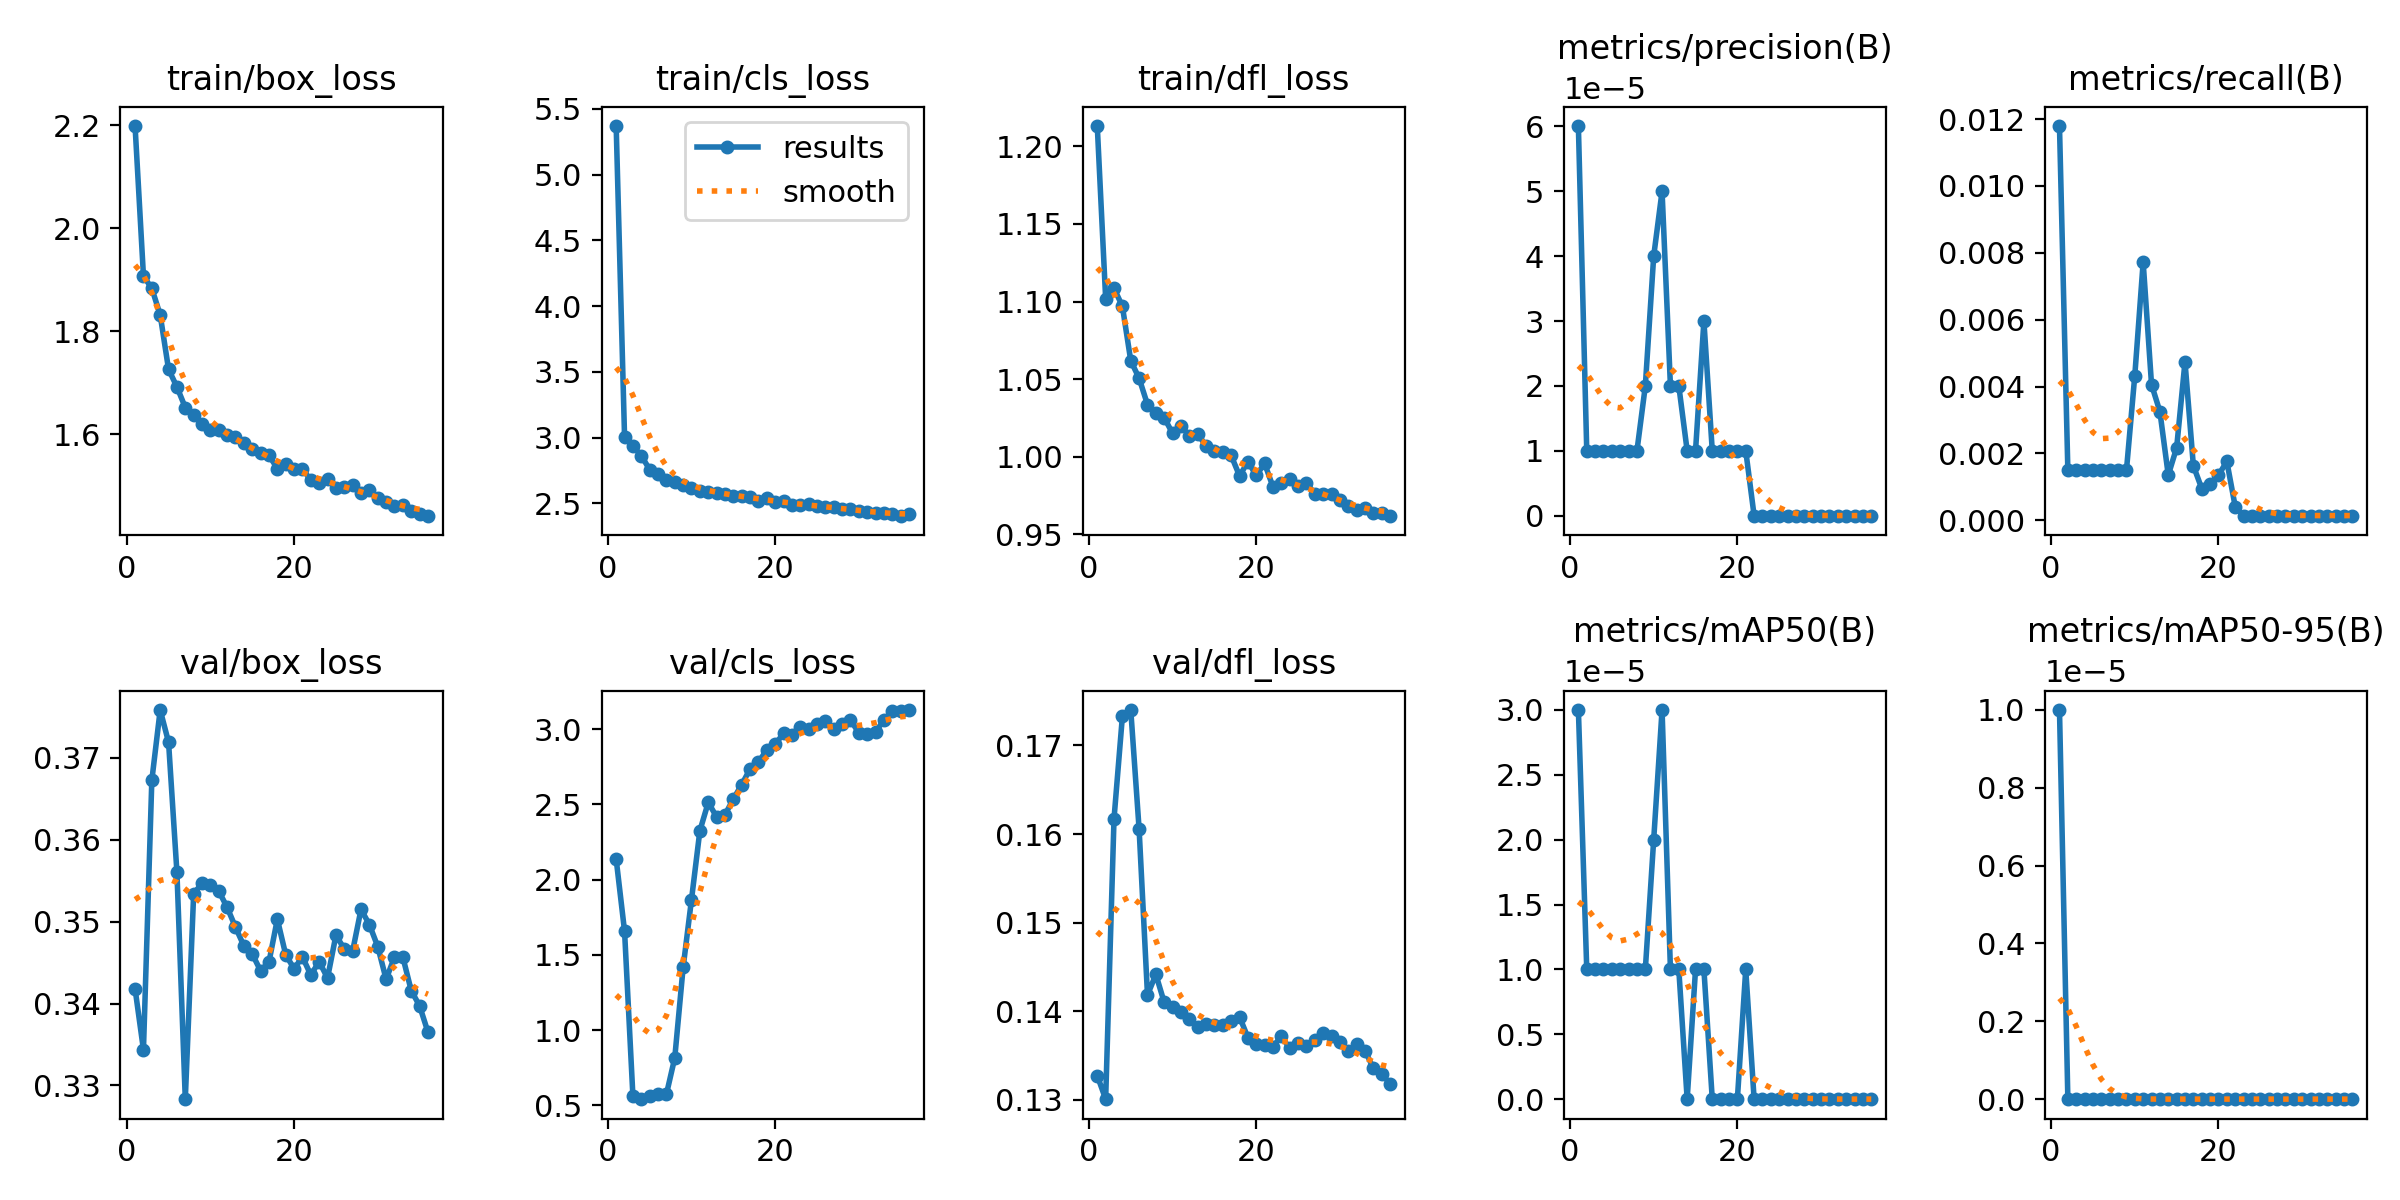
\includegraphics[width=0.75\textwidth]{images/results/hsv_results.png}
    \caption{Results of the model training with HSV data}
    \label{fig:results_hsv}
\end{figure}

% TODO results of hsv

% HSV + background subtraction
The HSV data was then combined with the background subtraction method. The results of this training are shown in Table~\ref{fig:results_hsv_backsub}.

\begin{figure}[htbp] 
    \centering
    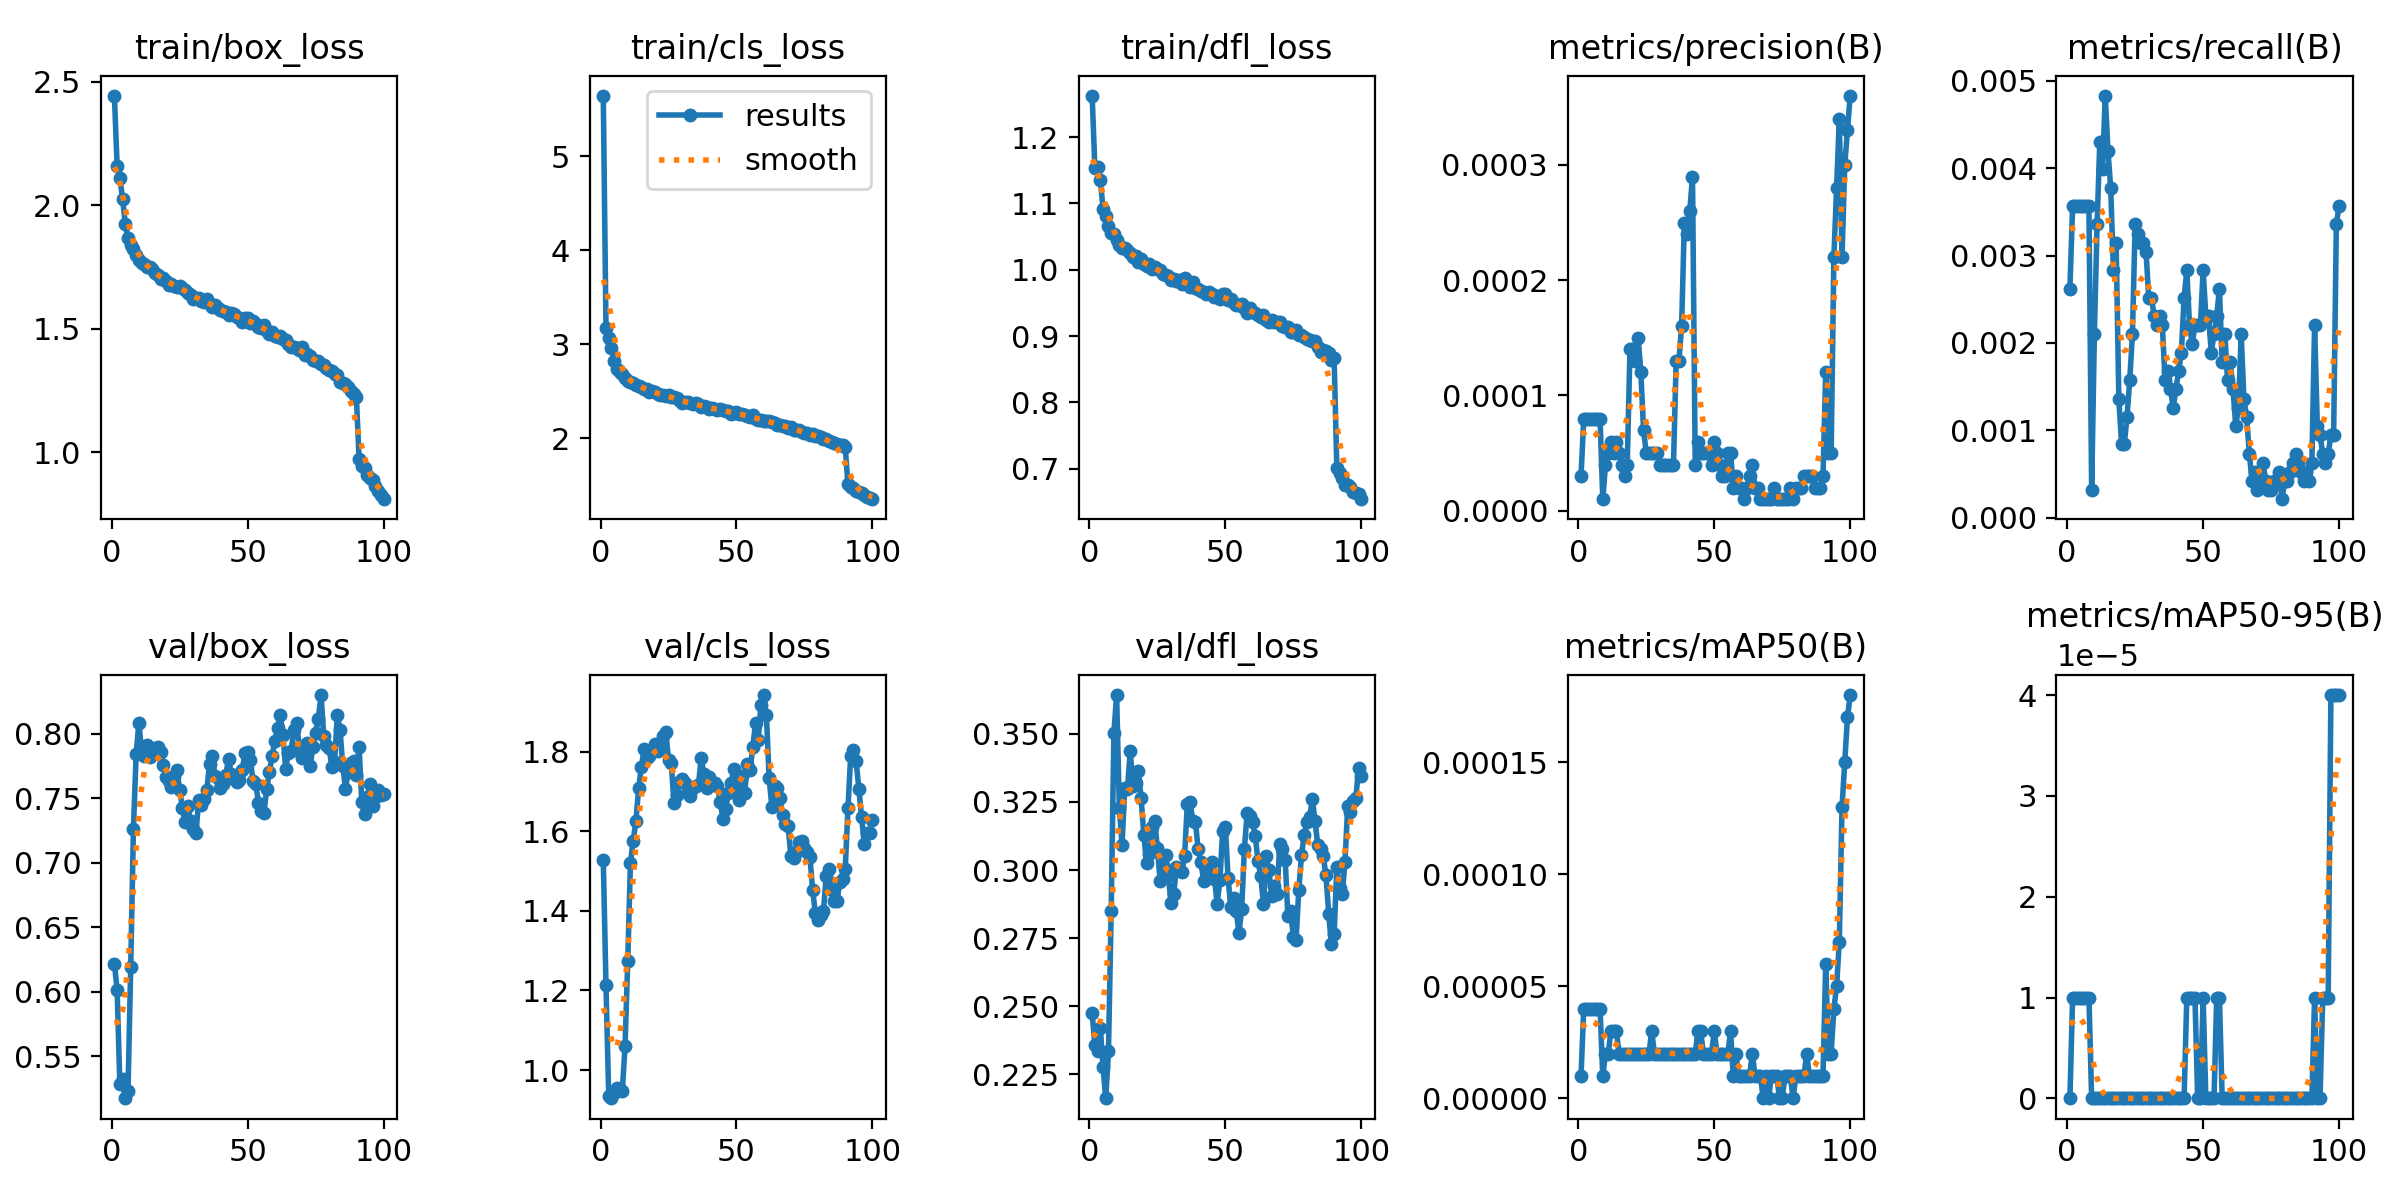
\includegraphics[width=0.75\textwidth]{images/results/hsv_bgsub_results.png}
    \caption{Results of the model training with HSV data and background subtraction}
    \label{fig:results_hsv_bgsub}
\end{figure}

% TODO results of hsv + background subtraction

% background subtraction

The background subtraction method was then used on its own. The results of this training are shown in Table~\ref{fig:results_bgsub}.

\begin{figure}[htbp] 
    \centering
    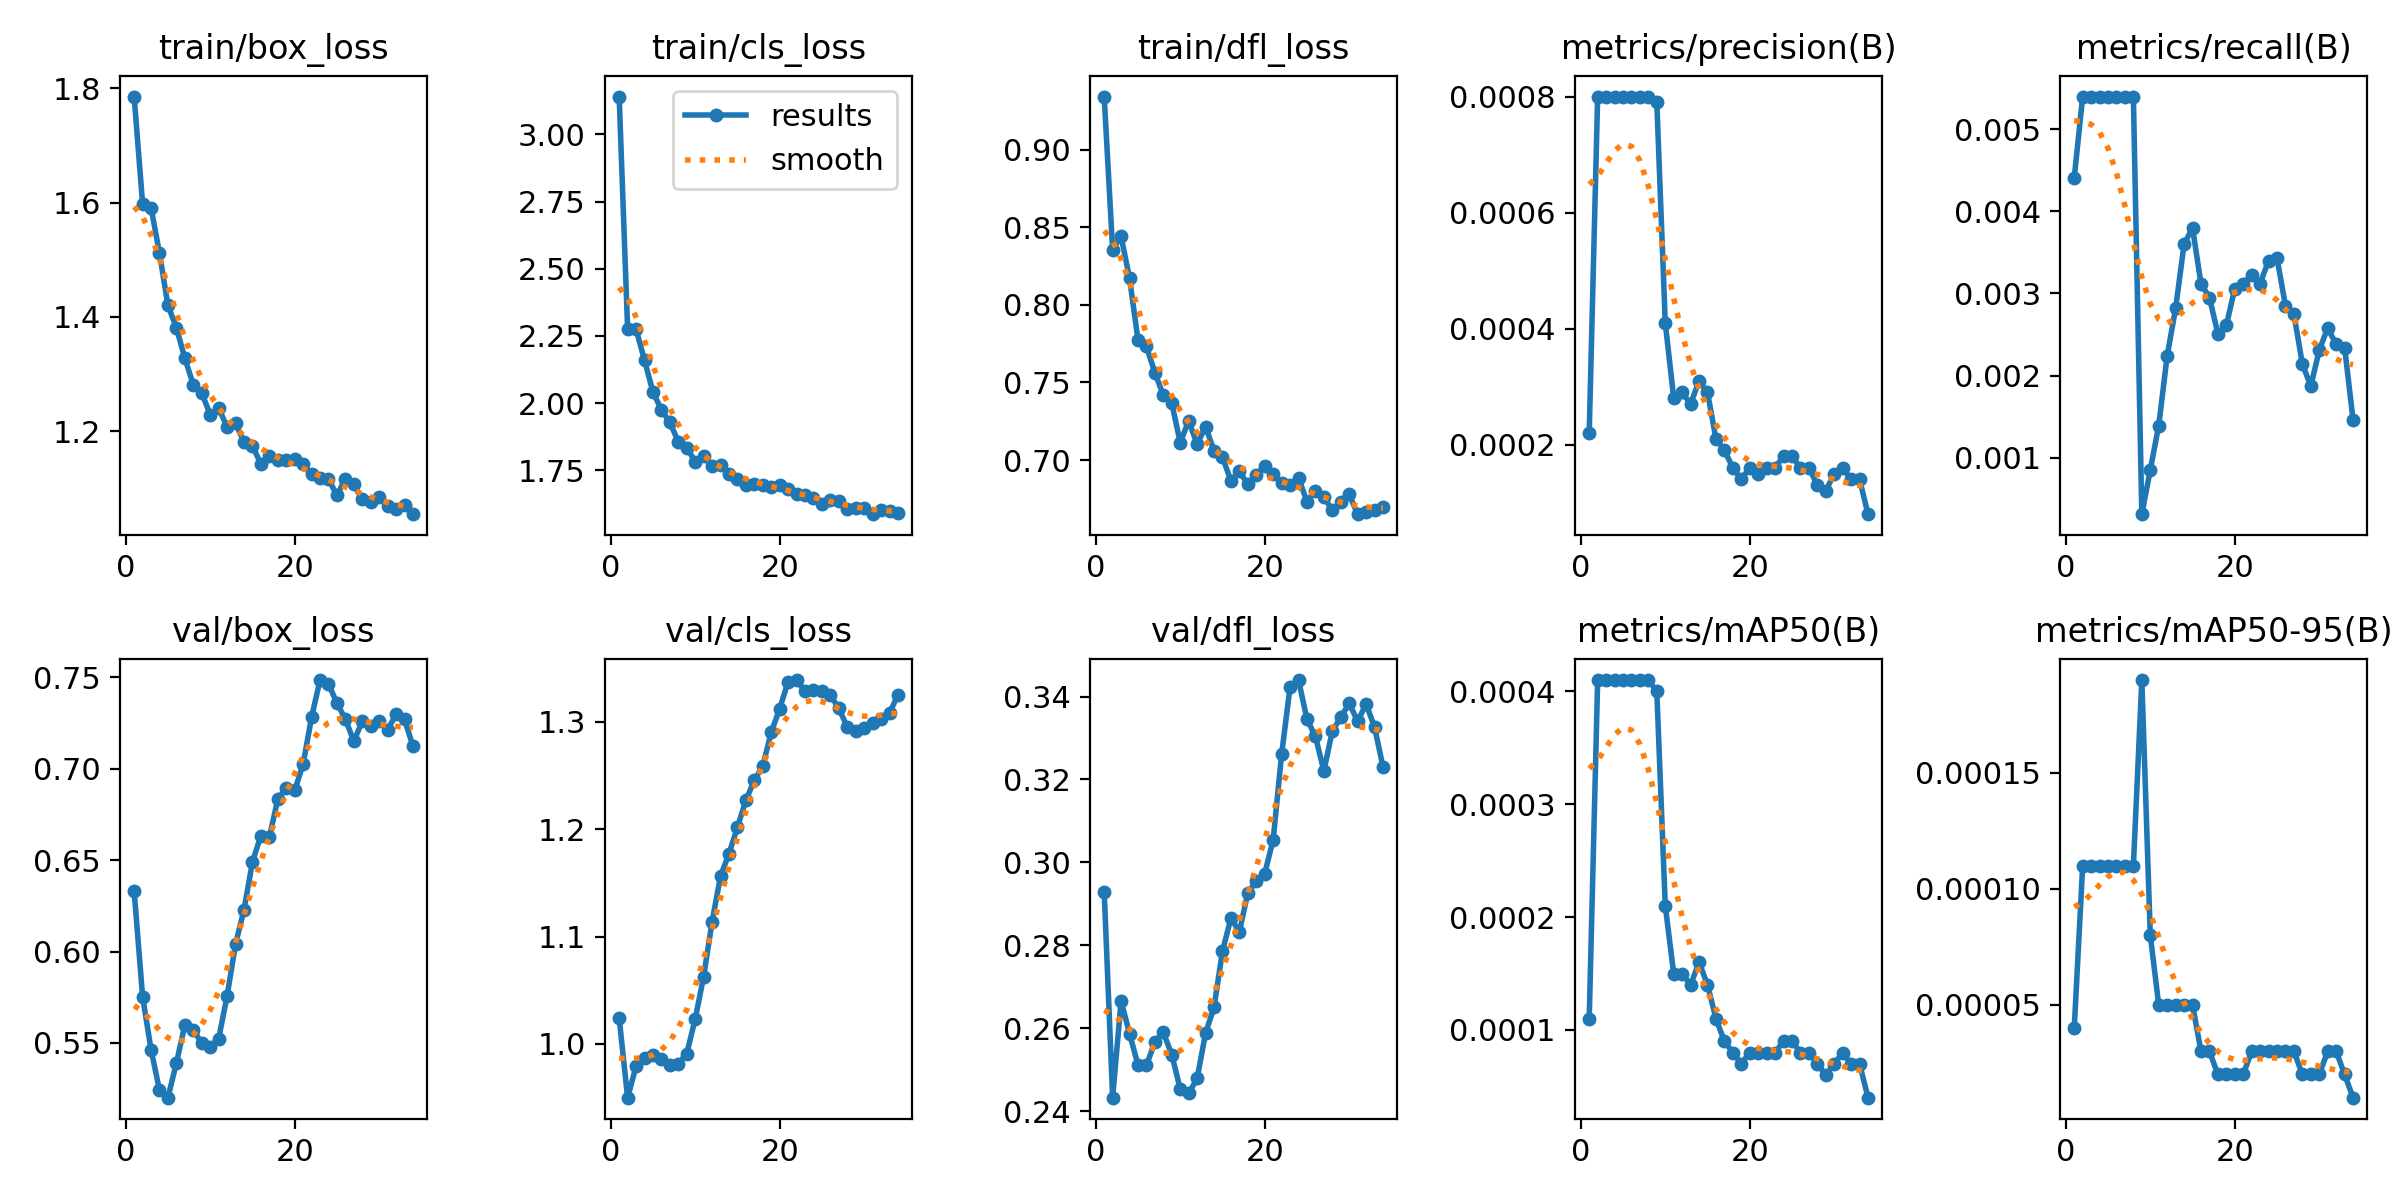
\includegraphics[width=0.75\textwidth]{images/results/bgsub_results.png}
    \caption{Results of the model training with background subtraction}
    \label{fig:results_bgsub}
\end{figure}

% TODO results of background subtraction

% background subtraction + time offset 1

The background subtraction method was then combined with the time offset method with an offset of 1. The results of this training are shown in Table~\ref{fig:results_bgsub_timeoffset1}.

\begin{figure}[htbp] 
    \centering
    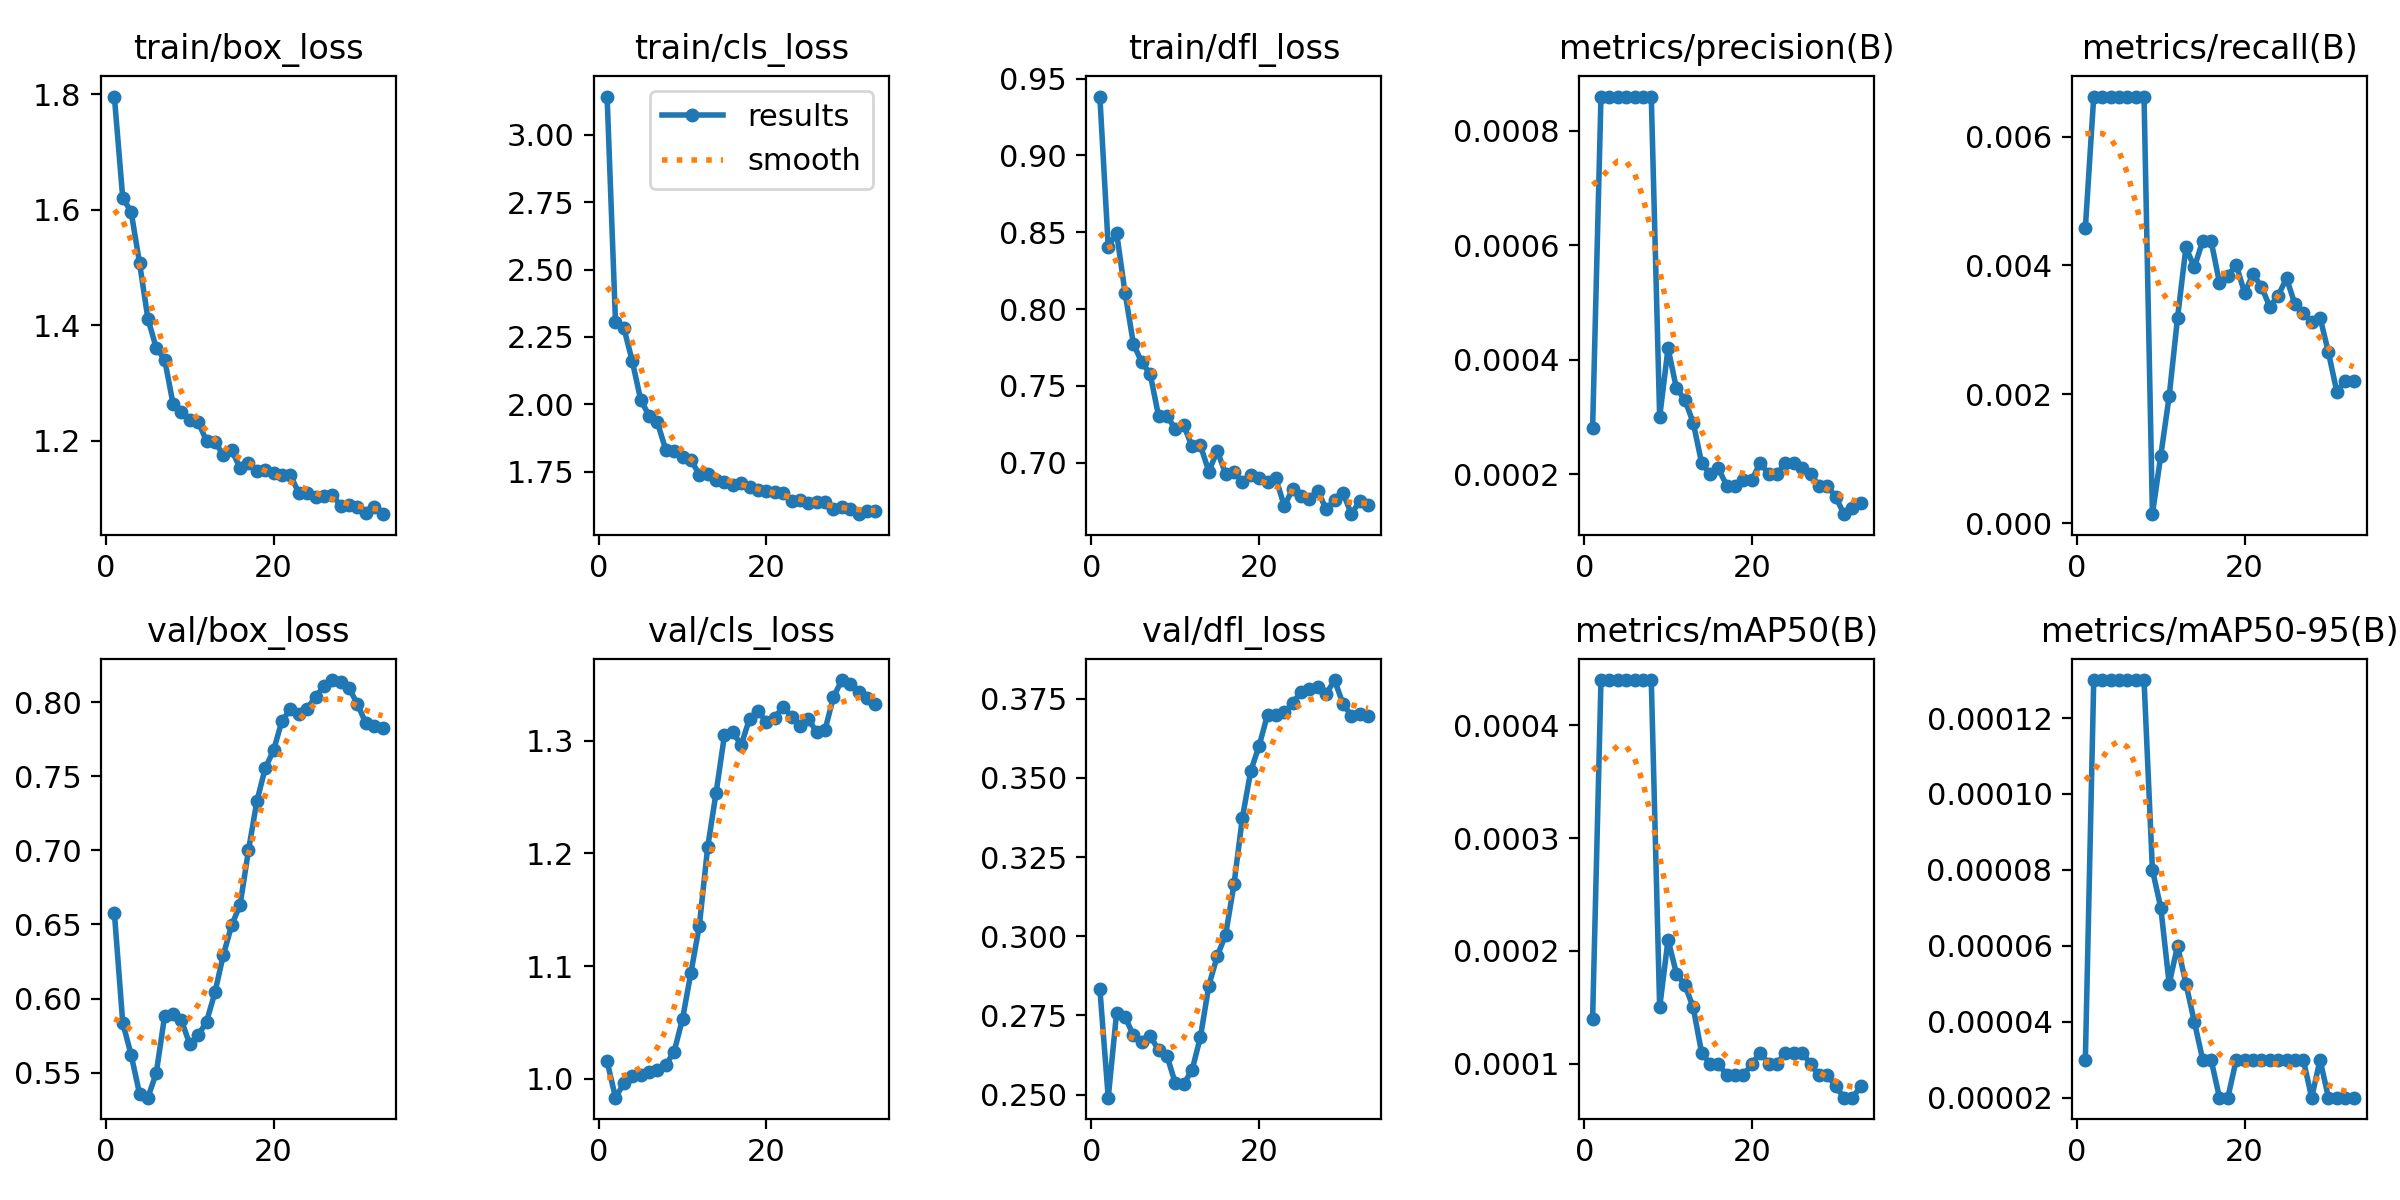
\includegraphics[width=0.75\textwidth]{images/results/bgsub_timeoffset1_results.png}
    \caption{Results of the model training with background subtraction and time offset 1}
    \label{fig:results_bgsub_timeoffset1}
\end{figure}

% TODO results of background subtraction + time offset 1